\section{Some Additional Security Settings}

Thunderbird provides additional security measures to protect you from
junk mail, identity theft, viruses (with the help of your anti-virus
software, of course), intellectual property theft, and malicious web
sites.

We will look at the following Thunderbird security features. First a
little background on why you need to consider some of these measures:

\begin{itemize}
\item
  \textbf{Adaptive junk mail controls}. Adaptive junk mail controls
  allow you to train Thunderbird to identify junk email (SPAM) and
  remove it from your inbox. You can also mark messages as junk mail
  manually if your email provider's system misses the junk mail and lets
  it go through.
\item
  \textbf{Integration with anti-virus software.} If your anti-virus
  software supports Thunderbird, you can use that software to quarantine
  messages that contain viruses or other malicious content. If you're
  wondering what anti-virus software works with Thunderbird, you can
  find a list here: http://kb.mozillazine.org/Antivirus\_software.
\item
  \textbf{Master password.} For your convenience, you can have
  Thunderbird remember each of your individual passwords of your e-mail
  accounts. You can specify a master password that you enter each time
  you start Thunderbird. This will enable Thunderbird to open all your
  email accounts with your saved passwords.
\item
  \textbf{Restrictions on cookies.} Some blogs and websites attempt to
  send cookies (a piece of text that stores information from Web sites
  on your computer) with their RSS feeds. These cookies are often used
  by content providers to provide targeted advertising. Thunderbird
  rejects cookies by default, but you can configure Thunderbird to
  accept some or all cookies.
\end{itemize}
In the Security Preferences section of Thunderbird's Options/Preferences
dialog box you can set up the preferences for these features.

\begin{itemize}
\item
  In Windows and Mac OS X, go to the `Tools' menu and click `Options'.
\item
  On Ubuntu or other versions of Linux, go to the `Edit' menu and click
  `Preferences'.
\end{itemize}
\subsection{Junk mail settings}

\begin{enumerate}[1.]
\item
  In the Preferences/Options dialog box, click `Security' and then click
  the `Junk' tab.
\end{enumerate}
\begin{figure}[htbp]
\centering
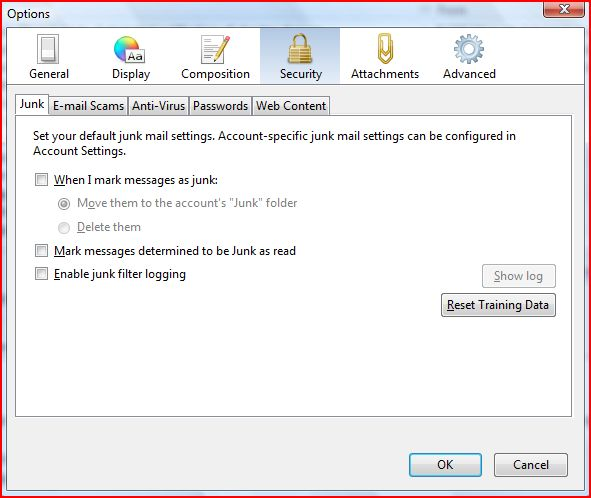
\includegraphics{thunderbird_sec_1.jpg}
\caption{Thunderbird Security}
\end{figure}

\begin{enumerate}[1.]
\setcounter{enumi}{1}
\item
  Do the following:
  \begin{itemize}
  \item
    To tell Thunderbird that it should handle messages marked as junk,
    select the check box labelled `When I mark message as junk'.
  \item
    To have Thunderbird move these messages to a junk folder, select the
    `Move them to account's 'Junk' folder' radio button.
  \item
    To have Thunderbird delete junk mail upon receiving it, select the
    `Delete them' radio button.
  \end{itemize}
\item
  Thunderbird will mark junk message as read if you select the check box
  labeled `Mark messages determined to be Junk as read'.
\item
  If you want to keep a log of junk mail received, select the `Enable
  junk filter logging' check box.
\item
  Click the `OK' button to close the `Options/Preferences' dialog box.
\end{enumerate}
\subsection{Scam detection and warning system}

\begin{enumerate}[1.]
\item
  In the Preferences/Options dialog box, click `Security' and then click
  the `E-mail Scams' tab.
\end{enumerate}
\begin{figure}[htbp]
\centering
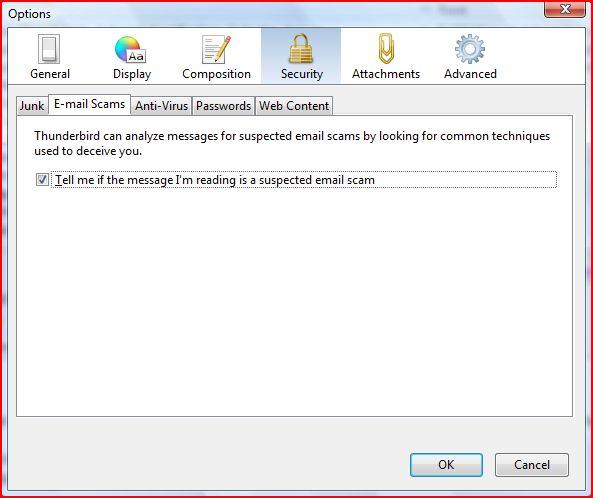
\includegraphics{thunderbird_sec_2.jpg}
\caption{Thunderbird Security}
\end{figure}

\begin{enumerate}[1.]
\setcounter{enumi}{1}
\item
  To have Thunderbird warn you about possible email scams, select the
  check box labelled `Tell me if the message I'm read is a suspected
  email scam'. To turn off this feature, deselect this check box.
\item
  Click the `OK' button to close the `Options/Preferences' dialog box.
\end{enumerate}
\subsection{Anti-virus integration}

\begin{enumerate}[1.]
\item
  In the Preferences/Options dialog box, click `Security' and then click
  the `Anti-Virus' tab.
\end{enumerate}
\begin{figure}[htbp]
\centering
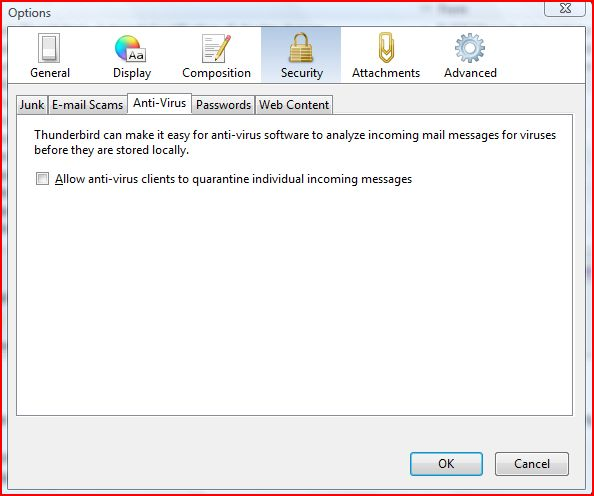
\includegraphics{thunderbird_sec_3.jpg}
\caption{Thunderbird Security}
\end{figure}

\begin{enumerate}[1.]
\setcounter{enumi}{1}
\item
  To turn on anti-virus integration, select the check box labeled `Allow
  anti-virus clients to quarantine individual incoming messages'. To
  turn off this feature, deselect this check box.
\item
  Click the `OK' button to close the `Options/Preferences' dialog box.
\end{enumerate}
\subsection{Set a master password}

\begin{enumerate}[1.]
\item
  In the Preferences/Options dialog box, click `Security' and then click
  the `Passwords' tab.
\end{enumerate}
\begin{figure}[htbp]
\centering
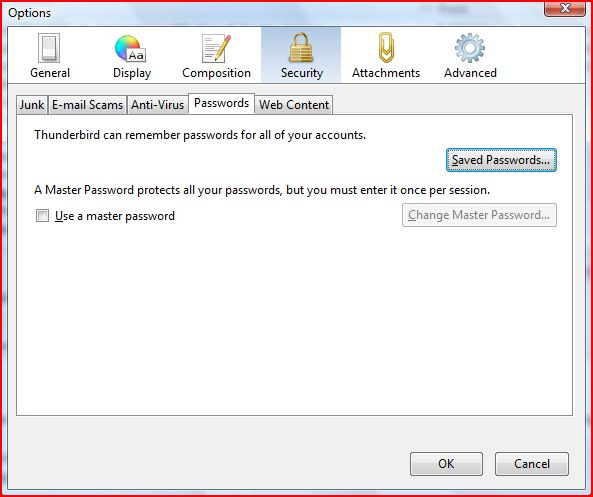
\includegraphics{thunderbird_sec_4.jpg}
\caption{Thunderbird Security}
\end{figure}

\begin{enumerate}[1.]
\setcounter{enumi}{1}
\item
  Select the check box labeled `Use a master password'.
\item
  Enter your password into the `Enter new password' and `Re-enter
  password' fields.
\end{enumerate}
\begin{figure}[htbp]
\centering
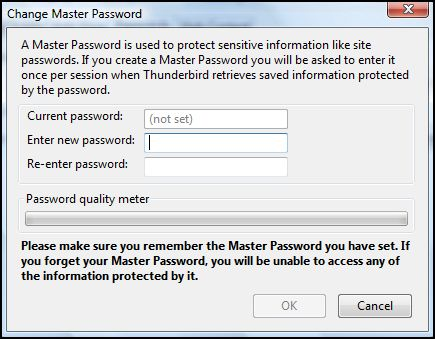
\includegraphics{thunderbird_sec_5.jpg}
\caption{Thunderbird Security}
\end{figure}

\begin{enumerate}[1.]
\setcounter{enumi}{3}
\item
  Click the `OK' button to close the Change Master Password dialog box.
\item
  If you want to see the passwords that you have saved in Thunderbird,
  click the `Saved Passwords' button. This will open the `Saved
  Passwords' dialog box.
\end{enumerate}
\begin{figure}[htbp]
\centering
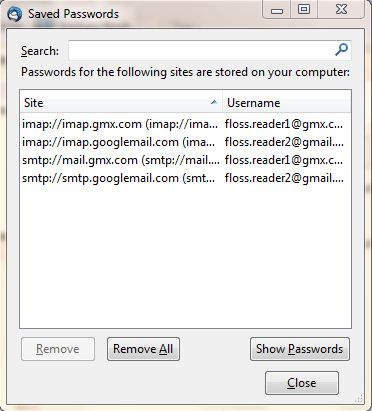
\includegraphics{thunderbird_sec_6.jpg}
\caption{Thunderbird Security}
\end{figure}

\begin{enumerate}[1.]
\setcounter{enumi}{5}
\item
  To see the passwords, click the `Show Passwords' button.
\end{enumerate}
\begin{figure}[htbp]
\centering
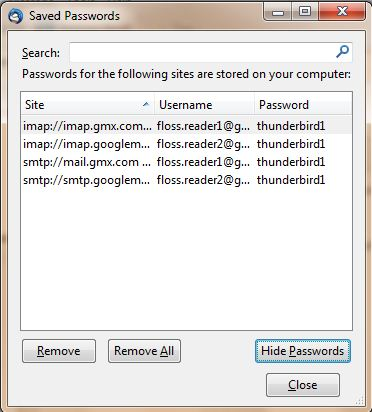
\includegraphics{thunderbird_sec_7.jpg}
\caption{Thunderbird Security}
\end{figure}

\begin{enumerate}[1.]
\setcounter{enumi}{6}
\item
  Click the `Close' button to close `Saved Passwords' dialog box.
\item
  Click the `OK' button to close the `Options/Preferences' dialog box.
\end{enumerate}
\subsection{Adaptive junk mail controls}

You need to first open Account Settings window. Note that settings
configured in the Account Settings window apply only to the account that
you select in the Folders pane. You must configure local folders
separately.

\begin{enumerate}[1.]
\item
  In the Folders pane right-click on an account name and select
  `Settings'.
\end{enumerate}
\begin{figure}[htbp]
\centering
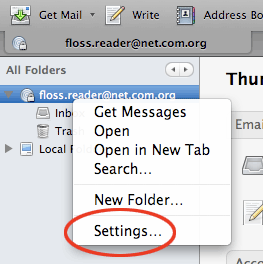
\includegraphics{thunderbird_sec_8.jpg}
\caption{Thunderbird Security}
\end{figure}

\begin{enumerate}[1.]
\setcounter{enumi}{1}
\item
  In Windows or Mac go to the `Tools' menu and select `Account
  Settings'. In Linux, go to the `Edit menu' and select `Account
  Settings'.
\item
  To set adaptive junk mail controls for a specific account, pick an
  account and click `Junk Settings'.
\end{enumerate}
\begin{figure}[htbp]
\centering
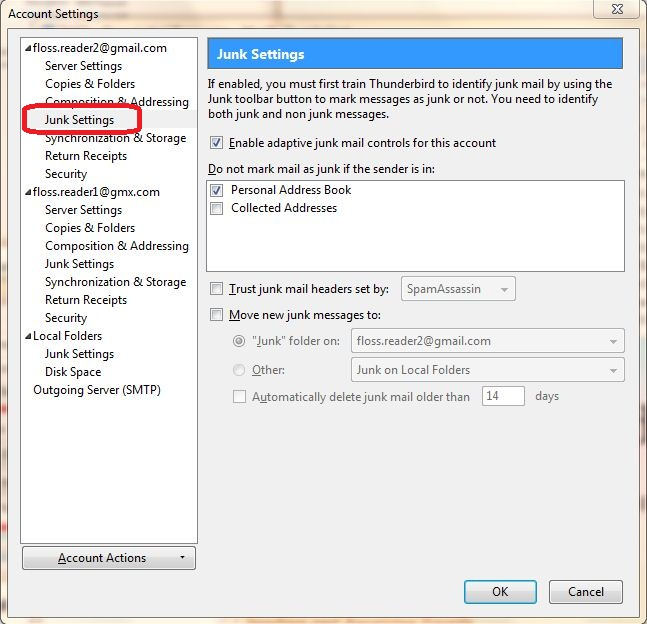
\includegraphics{thunderbird_sec_9.jpg}
\caption{Thunderbird Security}
\end{figure}

\begin{enumerate}[1.]
\setcounter{enumi}{3}
\item
  To turn on the controls, select the check box labeled `Enable adaptive
  junk mail controls for this account'. To turn them off, deselect this
  check box.
\item
  If you want the controls to ignore mail from senders in your Address
  Book, select the check boxes next to any of the listed address books.
\item
  To use a mail filter such as SpamAssassin or SpamPal, select the check
  box labelled `Trust junk mail headers sent by:' and pick a filter from
  the menu.
\item
  Select the check box labeled `Move new junk messages to' if you want
  to move junk mail to a specified folder. Then select the destination
  folder to be either at your email provider or a local folder on your
  computer.
\item
  Select the `Automatically delete junk mail other 14 days' check box to
  have Thunderbird regularly remove junk mail. To change the time period
  for this process, enter a different number (in days) in the text box.
\item
  Click `OK' to save your changes.
\end{enumerate}
